\begin{figure}[htpb]
\centering
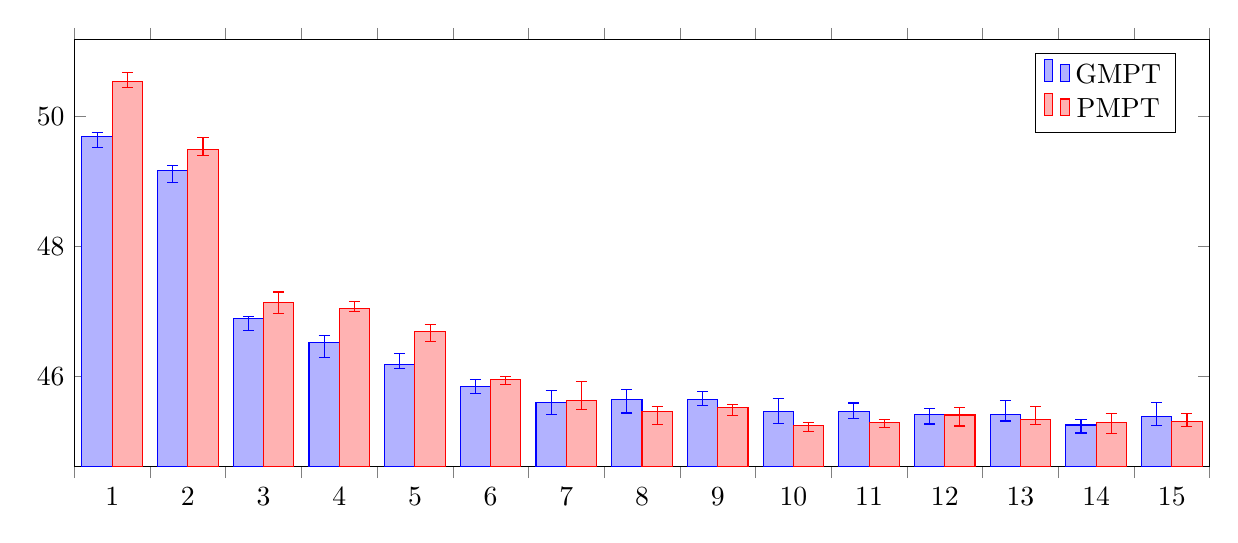
\begin{tikzpicture}
\begin{axis}[
legend pos=north east,
enlargelimits={abs=0.5},
ybar=0pt,
bar width=0.4,
width=16cm,
height=7cm,
xtick={0.5,1.5,...,15.5},
xticklabels={1,...,15},
x tick label as interval
]

\addplot+[error bars/.cd,
y dir=both,y explicit]
coordinates {
    (1,49.68478405) += (0,0.069966455) -= (0,0.168750135)
    (2,49.17207241) += (0,0.07217512) -= (0,0.19090019)
    (3,46.89177851) += (0,0.03515937) -= (0,0.18068561)
    (4,46.5205421) += (0,0.114861455) -= (0,0.229218385)
    (5,46.18018307) += (0,0.17726574) -= (0,0.06153901)
    (6,45.84314179) += (0,0.11067705) -= (0,0.10658501)
    (7,45.59441339) += (0,0.1838183) -= (0,0.17571021)
    (8,45.63928416) += (0,0.156660595) -= (0,0.201670185)
    (9,45.64222696) += (0,0.123004415) -= (0,0.089043455)
    (10,45.46320787) += (0,0.196236365) -= (0,0.189138275)
    (11,45.4666685) += (0,0.124598495) -= (0,0.119399435)
    (12,45.41869495) += (0,0.091439525) -= (0,0.149864225)
    (13,45.41417376) += (0,0.22016078) -= (0,0.09827707)
    (14,45.25437993) += (0,0.077996965) -= (0,0.123072465)
    (15,45.3839802) += (0,0.216019995) -= (0,0.142294955)};
\addplot+[error bars/.cd,
y dir=both,y explicit]
coordinates {
    (1,50.52727257) += (0,0.147734835) -= (0,0.080893685)
    (2,49.49040623) += (0,0.181165205) -= (0,0.095566265)
    (3,47.14078462) += (0,0.156947985) -= (0,0.168154885)
    (4,47.04225844) += (0,0.10671934) -= (0,0.0404122)
    (5,46.68459193) += (0,0.112148575) -= (0,0.143971945)
    (6,45.94851141) += (0,0.052713495) -= (0,0.074132765)
    (7,45.63239278) += (0,0.293799865) -= (0,0.139357765)
    (8,45.46463671) += (0,0.079556745) -= (0,0.206081505)
    (9,45.51780834) += (0,0.046734285) -= (0,0.116654175)
    (10,45.24352346) += (0,0.0486116) -= (0,0.09059746)
    (11,45.29471239) += (0,0.045160185) -= (0,0.084330065)
    (12,45.40729075) += (0,0.119223745) -= (0,0.169417925)
    (13,45.3325583) += (0,0.208028515) -= (0,0.066516575)
    (14,45.29665749) += (0,0.13401067) -= (0,0.17934347)
    (15,45.30736255) += (0,0.123567815) -= (0,0.081026515)};
\legend{GMPT,PMPT}
\end{axis}
\end{tikzpicture}
\caption[Comparison Single-Task Raspberry]{Comparison\footnotemark of the temperature measurements for GMPT and PMPT}
\label{fig:i_eva_sabar_pi}
\end{figure}
\footnotetext{The bar values correspond to the median and the error bars correspond to the lower and upper inner fences displayed in the boxplots in \autoref{fig:i_eva_sabar_pi}}